% Ci sono iniziative che per l'enabling di calcolo numerico anche complesso sul client web
% poi spiego il modo
%% spiego da dove arriva
%% immagine di come funziona (plugin)

With the advent of \ac{GPGPU}, the spreading of multicore CPUs and multiprocessor
programming (like OpenMP) we can see emerging an intersection in parallel computing.
This intersection is known as \textbf{heterogeneus computing}. There are
initiatives aimed at enabling numeric calculation, even complex, on the web client.
\ac{OpenCL} is a framework for heterogeneus computing and \ac{WebCL} is a porting
of this technlogy to the web.\\

\begin{figure}[htb]
    \centering
    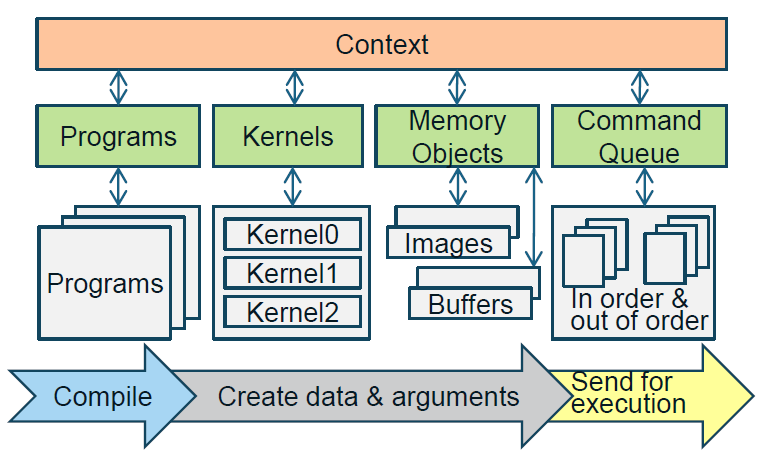
\includegraphics[width=\columnwidth]{opencl}
    \caption{OpenCL execution flow.}
    \label{fig:opencl}
\end{figure}
\ac{OpenCL} execution is based on \emph{kernels}, special functions written in
a language based on C99\footnote{A programming language dialect for the past C
developed in 1999 (formal name ISO/IEC 9899:1999)} with some extensions. These
\emph{kernels} can be compiled at build-time or at run-time and also have a rich
setof built-in function, e.g. \code{cross}, \code{dot}, \code{sin}, \code{cos},
\code{pow}, \code{log}, etc.

\begin{figure}[htb]
    \centering
    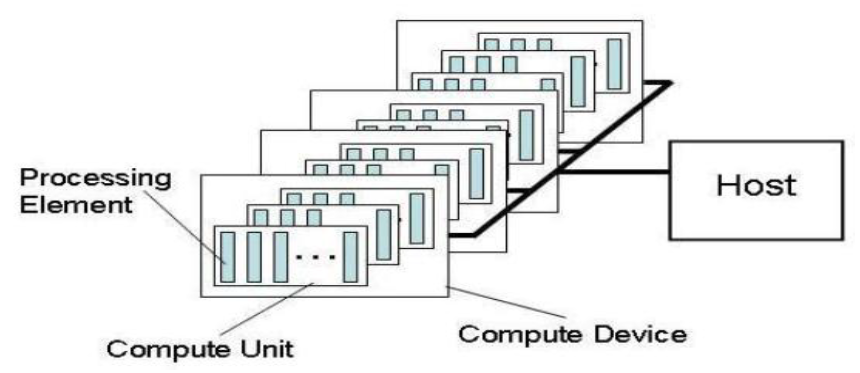
\includegraphics[width=\columnwidth]{opencl-device}
    \caption{OpenCL device composition.}
    \label{fig:opencl-device}
\end{figure}
An \ac{OpenCL} device (like CPU or GPU) is composed by (see
\autoref{fig:opencl-device}):
\begin{itemize}
    \item A collection of one or more \textbf{compute units}, this concept is
    similar to the \emph{cores} of a standard CPU.

    \item A \emph{compute unit} is composed by one or more \textbf{processing
    elements}, this concept is similar to the \emph{threads}.

    \item Processing elements execute code as \ac{SIMD} or \ac{SPMD}.
\end{itemize}

Once the \emph{kernels} have been created the flow for executing an \ac{OpenCL}
program can start. Here is the list of action performed to run code on
\ac{OpenCL} enabled computer:
\begin{enumerate}
    \item Query host for \ac{OpenCL} devices.
    \item Create a context to associate \ac{OpenCL} devices.
    \item Create programs for execution on one or more associated devices.
    \item From the programs, select kernels to execute.
    \item Create memory objects accessible from the host and/or the device.
    \item Copy memory data to the device as needed.
    \item Provide kernels to the command queue for execution.
    \item Copy results from the device to the host
\end{enumerate}

Currently there are two main implementation of this API, one supporting Windows
and Linux using Firefox (holded by Nokia), and one, holded by Samsung, that
bring this interface to WebKit browsers. Speaking of performance improvements
\autoref{tab:webcl-speedup} shows the data from the TIZEN\tm{} developer
conference held in May 2012:
\begin{table}[h!tb]
    \caption{Samsung WebCL performance compared to pure \js{}.}
    \label{tab:webcl-speedup}
    \centering
    \begin{tabular}{r|c|c|c}
        \textbf{Demo name} & \textbf{\js{}} & \textbf{WebCL} & \textbf{Speed-up}\\
        \hline
        Sobel filter (with 256x256 image) & $\sim{}$200ms & $\sim{}$15ms & 13x\\
        \hline
        N-body simulation (1024 particles) & 5-6fps & 75-115fps & 12-23x\\
        \hline
        Deformation (2880 vertices) & $\sim{}$1fps & 87-116fps & 87-116x
    \end{tabular}
\end{table}
